\documentclass[runningheads,a4paper]{llncs}
\usepackage{fontspec}
\usepackage{polyglossia}
\setdefaultlanguage{russian}
\setotherlanguage{english}
\setmainfont{cmunrm.otf}[BoldFont=cmunbx.otf,ItalicFont=cmunti.otf,BoldItalicFont=cmunbi.otf]
\setsansfont{cmunss.otf}[BoldFont=cmunsx.otf,ItalicFont=cmunsi.otf,BoldItalicFont=cmunso.otf]
\setmonofont{cmuntt.otf}[BoldFont=cmuntb.otf,ItalicFont=cmunit.otf]
\newfontfamily\cyrillicfont{cmunrm.otf}[BoldFont=cmunbx.otf,ItalicFont=cmunti.otf,BoldItalicFont=cmunbi.otf]
\newfontfamily\cyrillicfontsf{cmunss.otf}[BoldFont=cmunsx.otf,ItalicFont=cmunsi.otf,BoldItalicFont=cmunso.otf]
\newfontfamily\cyrillicfonttt{cmuntt.otf}[BoldFont=cmuntb.otf,ItalicFont=cmunit.otf]
\usepackage{microtype,graphicx,booktabs,tabularx,array,amsmath,amssymb,xcolor}
\usepackage{hyperref}
\newcolumntype{L}{>{\raggedright\arraybackslash}X}
\graphicspath{{figures/}}
\hypersetup{hidelinks,pdftitle={Углублённая доразметка и контролируемые пулы кандидатов в переоценке моделей ранжирования на коллекции MS MARCO},pdfauthor={, , }}
\setlength{\emergencystretch}{1.5em}
\setlength{\tabcolsep}{4pt}
\renewcommand{\arraystretch}{1.12}
% Generated by build_tables.py from evaluation summaries.
\newcommand{\ManualQueryCount}{1\,179}
\newcommand{\ManualPairCount}{33\,667}
\newcommand{\FullQueryCount}{101\,093}
\newcommand{\JudgeTestAuc}{0.907}
\newcommand{\JudgeTestFOne}{0.875}
\newcommand{\JudgeTestPrecision}{0.851}
\newcommand{\JudgeTestRecall}{0.902}
\newcommand{\JudgeHeldoutOriginalNdcg}{0.512}
\newcommand{\JudgeHeldoutHumanNdcg}{0.938}
\newcommand{\FullPositiveLargeConditional}{130.70}
\newcommand{\OriginalPositiveCount}{1\,243}
\newcommand{\OriginalMeanRel}{1.05}
\newcommand{\HumanPositiveCount}{20\,597}
\newcommand{\HumanMeanRel}{17.47}
\newcommand{\JudgePositiveCount}{22\,206}
\newcommand{\JudgeMeanRel}{18.83}
\newcommand{\BmOriginal}{0.248}
\newcommand{\BmHuman}{0.644}
\newcommand{\EOriginal}{0.488}
\newcommand{\EHuman}{0.879}
\newcommand{\FullPoolSmall}{21.88}
\newcommand{\FullPositiveSmall}{14.19}
\newcommand{\FullPoolLarge}{451.54}
\newcommand{\FullPositiveLarge}{128.64}

\title{Углублённая доразметка и контролируемые пулы кандидатов в переоценке моделей ранжирования на коллекции MS MARCO}
\titlerunning{Углублённая доразметка и контролируемые пулы кандидатов}
\author{}
\authorrunning{}
\institute{}

\begin{document}
\maketitle
\begin{abstract}
При оценке поисковых систем неполная разметка релевантности может оставлять правильные ответы неучтёнными. Мы исследуем дополнительную ручную разметку английской MS MARCO на \ManualQueryCount{} запросах и \ManualPairCount{} парах «запрос--фрагмент» из объединённого пула. Углублённая доразметка здесь означает оценку нескольких кандидатов в заданном пуле без предположения, что исходный положительный фрагмент исчерпывает релевантные ответы. При неизменном ранжировании среднее число положительных меток на запрос возрастает с \OriginalMeanRel{} до \HumanMeanRel{}. При общей нормировке по пулу и одинаковом наборе запросов NDCG@10 увеличивается с \BmOriginal{} до \BmHuman{} для BM25 и с \EOriginal{} до \EHuman{} для E5. Компактная модель-судья типа cross-encoder достигает ROC-AUC \JudgeTestAuc{} на отложенных данных и используется для псевдоразметки \FullQueryCount{} запросов. Мы пересчитываем эти метки по сохранённым оценкам с фиксированным порогом и анализируем глубину пула от 10 до 200. Отбор кандидатов меняет как охват разметки, так и интерпретацию результатов объединения рангов. Выводы относятся к исследованным пулам и не означают ни исчерпывающей разметки корпуса, ни переносимости между поисковыми провайдерами и группами пользователей.
\keywords{информационный поиск \and MS MARCO \and оценки релевантности \and доразметка \and формирование пула \and объединение по обратным рангам}
\end{abstract}

\section{Введение}
\label{sec:intro}

Для оценки информационного поиска нужны запросы, документы и суждения о том, какие документы удовлетворяют каждому запросу. MS MARCO, широко используемая коллекция, построена на реальных поисковых запросах Bing \cite{bajaj2016msmarco}. Для задачи ранжирования фрагментов текста доступны тексты запросов и фрагментов и неполная разметка релевантности, обычно называемая \emph{qrels} (query relevance judgments) \cite{msmarco_datasets}. Для большинства запросов в размеченной подвыборке разработки указан лишь один положительный фрагмент. Другие подходящие ответы могут оставаться неразмеченными и потому не давать вклада в метрику.

MS MARCO представляет одного из нескольких поисковых провайдеров, а не универсальную выборку информационных потребностей. Natural Questions от Google содержит реальные поисковые запросы и ручную разметку ответов на страницах Wikipedia \cite{kwiatkowski2019naturalquestions}. В Learning to Rank Challenge от Yahoo! опубликованы два набора векторов признаков пар «запрос--документ» с градуированными оценками релевантности, но без текстов запросов и документов \cite{chapelle2011yahoo}. В Personalized Web Search Challenge от Yandex опубликованы журналы сессий и кликов с анонимизированными идентификаторами вместо читаемых запросов и документов \cite{yandex2013personalized}. Эти коллекции также полезны для исследований поиска, но их задачи и представления данных отличаются от задачи ранжирования фрагментов.

Мы выбрали MS MARCO, поскольку доступные тексты, неполная ручная разметка, устоявшиеся средства оценки и предобученные модели позволяют сопоставлять результаты с предшествующими работами. Неполнота разметки также позволяет непосредственно исследовать эффект её расширения. Этот выбор не предполагает универсальности: на переносимость могут влиять особенности выборки провайдера, язык, намерения пользователей и предметная область документов. Различия между странами и социальными группами в работе не измеряются.

Под \emph{углублённой доразметкой} мы понимаем расширение оценок релевантности на документы-кандидаты в заданном пуле. «Углублённая» характеризует охват разметки, а не глубину нейронной сети или повторное обучение. Это не означает исчерпывающей оценки всего корпуса. Например, для запроса о причинах повышения температуры кипения жидкости несколько фрагментов могут объяснять действие добавленной соли. Если в исходных qrels указан только один, другое верное объяснение не даёт вклада в метрику до его оценки. В разделе~\ref{sec:example} приведён реальный пример с идентификаторами фрагментов и метками до и после доразметки.

При сравнении исходной и ручной разметки ранжирование фиксировано. Поэтому рост измеренной NDCG после доразметки не означает улучшения самой поисковой модели: её неизменная выдача оценивается по более полной разметке. Во второй части исследования обученная модель-судья расширяет охват разметки на более крупные пулы кандидатов. Её предсказания называются \emph{псевдометками}, чтобы отличать их от человеческих оценок.

Мы рассматриваем три вопроса: (1) как дополнительная ручная разметка меняет охват оценок и измеряемое качество ранжирования; (2) насколько компактная модель-судья согласуется с отложенными человеческими оценками; (3) как на оценку влияют глубина пула и глубина входных списков метода объединения по обратным рангам (Reciprocal Rank Fusion, RRF) \cite{cormack2009rrf}. Вклад работы состоит в анализе решений о разметке и оценке, а не в новой архитектуре поиска.

\section{Связанные работы}
\label{sec:related}

MS MARCO используется для обучения и оценки нейросетевых поисковых моделей \cite{bajaj2016msmarco}. Коллекция mMARCO расширяет задачу ранжирования фрагментов на несколько языков посредством перевода \cite{bonifacio2022mmarco}; её русская часть также включена в RusBEIR \cite{2025rusbeir}. В наших экспериментах используются английские тексты запросов и фрагментов. За рамки одного провайдера выходит BEIR, оценивающий поиск на 18 наборах данных с разными задачами и предметными областями \cite{thakur2021beir}. Межколлекционная оценка исследует переносимость между наборами данных, но сама по себе не устанавливает демографическую репрезентативность.

BM25, лексический базовый метод, учитывает совпадения и частоты терминов и нормировку по длине документа \cite{robertson2009bm25}. Плотные bi-encoder-модели, такие как E5 и BGE, независимо кодируют запрос и документ, затем сравнивают их векторы \cite{wang2022e5,xiao2023cpack}. Cross-encoder-модели обрабатывают запрос и кандидата совместно, учитывая взаимодействия токенов ценой больших вычислительных затрат \cite{nogueira2019bert}. Эти различия важны, поскольку разные системы могут добавлять в пул разные релевантные фрагменты.

Формирование пула (pooling) представляет собой стандартный способ построения тестовых коллекций: первые документы выдачи нескольких источников объединяются и оцениваются людьми \cite{voorhees2005trec}. Это сокращает трудоёмкость разметки, но ставит её охват в зависимость от систем-источников и глубины отбора. RRF объединяет входные ранги без обучения модели калибровки оценок \cite{cormack2009rrf}. Его поведение может зависеть от усечения списков, входных систем и параметров объединения \cite{bruch2023fusion}. Поэтому мы явно задаём и состав пула кандидатов, и списки, поступающие на объединение.

\section{Данные и ручная доразметка}
\label{sec:data}

\subsection{Исходная коллекция и пул кандидатов}

Английский корпус MS MARCO содержит 8\,841\,823 фрагмента. Используемые официальные qrels подвыборки разработки включают 7\,437 положительных пар для 6\,980 запросов \cite{msmarco_datasets}. Ручная подвыборка содержит \ManualQueryCount{} запросов и \ManualPairCount{} различных пар «запрос--фрагмент»: в среднем 28.56 кандидата на запрос, максимум 63. Более масштабный эксперимент с псевдоразметкой использует \FullQueryCount{} запросов с сохранёнными ранжированными списками; этот набор не совпадает с размеченной подвыборкой разработки из 6\,980 запросов.

Ручной пул сформирован объединением результатов поиска по запросу со вспомогательными каналами отбора кандидатов. Для каждого запроса сохранено по десять результатов BM25, E5 и BGE. Данные разметки также содержат вспомогательные каналы с именами \texttt{e5-rerank} и \texttt{s0}--\texttt{s3}. Они добавляют кандидатов сверх трёх списков поиска только по запросу. В частности, у 6\,258 пар нет оценки ни BM25, ни E5, ни BGE, ни \texttt{e5-rerank}; 35 пулов содержат более 40 документов. Таким образом, пул разметки включает дополнительных кандидатов за пределами четырёх названных списков первых десяти результатов.

При подготовке кандидатов также использовалось сходство с известным релевантным ответом, вычисленное с помощью E5 в рамках процедуры разметки с опорным ответом. Этот сигнал использует информацию об ответе, недоступную при обычном поиске только по запросу. Для анализа разметки сохраняется полный пул. Контролируемое сравнение ранжирования включает BM25, E5, BGE и их трёхсторонний RRF; вспомогательные каналы участвуют в пулинге, но исключены из сравнения систем, поскольку использованные в них модели не установлены. Для ранжирования полного набора используются \texttt{intfloat/e5-small-v2} и \texttt{BAAI/bge-small-en-v1.5}. Эти идентификаторы относятся к выдачам полного набора; точные конфигурации вспомогательных каналов ручного пула остаются неустановленными.

\subsection{Задача асессора}
\label{sec:annotation}

Для каждой отобранной пары асессор видел запрос, фрагмент-кандидат и исходный релевантный фрагмент MS MARCO. Требовалось определить, отвечает ли кандидат той же информационной потребности. Опорный фрагмент помогал согласовать интерпретацию с исходной разметкой, но не требовал повторять его формулировки. Формирование пула с последующими дополнительными оценками и составляет исследуемую углублённую доразметку.

В записях разметки различаются категория исходно положительных документов и новые положительные документы. Для неполной базовой разметки мы берём официальные qrels подвыборки разработки и пересекаем их с сохранённым пулом, а не выводим исходную релевантность из категории разметки. Это даёт \OriginalPositiveCount{} положительных пар. Четырнадцать пар, отмеченных как исходно положительные, но отсутствующих в официальных qrels, остаются в расширенной ручной разметке, однако не учитываются как официальные положительные пары.

Ручные положительные метки охватывают \HumanPositiveCount{} пар. Также имеются 13\,041 явная отрицательная оценка и 29 нестандартных значений категории с неустановленным смыслом. Последние оставлены неразмеченными: они дают нулевой вклад на исходных позициях ранжирования, но не считаются подтверждёнными отрицательными оценками. Пять полей с текстом фрагмента пусты. Анализ чувствительности исключает все 23 запроса с нестандартными метками или пустыми текстами. На оставшихся 1\,156 запросах сохраняются порядок систем и основной эффект доразметки (раздел~\ref{sec:manual-results}).

\begin{table}[t]
\caption{Охват разметки в одном и том же ручном пуле. Автоматические метки не являются дополнительными человеческими оценками.}
\label{tab:annotation-data}
\centering\small
\begin{tabularx}{\textwidth}{@{}Lrrr@{}}
\toprule
Показатель & Исходная & Ручная & Судья \\
\midrule
Запросов & 1\,179 & 1\,179 & 1\,179 \\
Пар в пуле & 33\,667 & 33\,667 & 33\,667 \\
Положительных пар & 1\,243 & 20\,597 & 22\,206 \\
Положительных на запрос, среднее & 1.05 & 17.47 & 18.83 \\
Положительных на запрос, медиана & 1 & 17 & 19 \\
\bottomrule
\end{tabularx}
\end{table}


Число запросов при ручной доразметке не увеличивается. Меняется число положительных оценок в том же пуле: среднее растёт с \OriginalMeanRel{} до \HumanMeanRel{}, медиана с 1 до 17. Эти величины характеризуют отобранные наборы кандидатов, а не общее число релевантных фрагментов в корпусе.

\subsection{Конкретный пример}
\label{sec:example}

Таблица~\ref{tab:example} иллюстрирует запрос 1086224 «what causes boiling point to increase» («что вызывает повышение температуры кипения»). Исходный положительный фрагмент объясняет, что добавление соли повышает температуру кипения. Второй фрагмент даёт то же релевантное объяснение через понятие «нелетучее растворённое вещество», но отсутствует в неполных qrels. Фрагмент с температурой кипения ацетона не объясняет запрошенную причину и в этом пуле имеет отрицательную ручную оценку.

\begin{table}[t]
\caption{Пример из ручной разметки. Описания фрагментов представляют собой сокращённый пересказ, а не новые оценки. «Не размечен» означает отсутствие в исходных положительных qrels.}
\label{tab:example}
\centering\small
\begin{tabularx}{\textwidth}{@{}l L l l@{}}
\toprule
ID фрагмента & Содержание & Исходно & Вручную \\
\midrule
7112148 & Добавление соли в воду повышает её температуру кипения. & Релевантен & Релевантен \\
7399382 & Добавление нелетучего растворённого вещества, например соли, повышает температуру кипения растворителя. & Не размечен & Релевантен \\
987600 & Указана температура кипения ацетона. & Не размечен & Нерелевантен \\
\bottomrule
\end{tabularx}
\end{table}

Пусть система возвращает фрагмент 7399382 первым. При неполной разметке он даёт нулевой вклад в метрику, хотя отвечает на вопрос. После ручной оценки его вклад становится положительным при неизменной выдаче. Пример разграничивает отсутствие оценки и ошибку поиска и показывает, почему важно учитывать несколько релевантных фрагментов на запрос. Он иллюстрирует процедуру, но не частоту конкретной ошибки во всей коллекции.

\section{Модель-судья и протокол оценки}
\label{sec:protocol}

\subsection{Назначение и вход модели-судьи}
\label{sec:judge-method}

Полная ручная оценка десятков миллионов отобранных пар практически неосуществима. Модель-судья переносит сигнал ручной разметки на более крупные пулы. BM25, E5 и BGE по-прежнему формируют кандидатов, а судья присваивает оценки релевантности уже отобранным парам. Поэтому согласие судьи с человеческими оценками следует устанавливать отдельно от эффективности поиска.

Мы используем компактную модель \texttt{cross-encoder/ms-marco-MiniLM-L6-v2} \cite{wang2020minilm,reimers2019sentencebert}.\footnote{\url{https://huggingface.co/cross-encoder/ms-marco-MiniLM-L6-v2}} Она обрабатывает запрос и фрагмент-кандидат совместно, в отличие от раздельного кодирования в E5 и BGE. На вход подаются только эти два текста, без поисковых эмбеддингов, рангов, оценок объединения или известного релевантного ответа. MiniLM выбрана как общедоступная и вычислительно доступная базовая модель для MS MARCO, а не как сильнейший из доступных судей релевантности.

В исходном эксперименте обучения все 1\,179 запросов разделены на 825 обучающих, 177 валидационных и 177 тестовых, содержащих соответственно 23\,543, 5\,122 и 5\,002 пары. Разбиение выполнено перемешиванием групп по запросам с seed 42, поэтому один запрос не может попасть в разные части. Дообучение проводилось в течение двух эпох с размером батча 16, максимальной длиной последовательности 512 и 100 шагами разогрева. В том запуске категории 1 и 2 считались положительными, остальные преобразовывались в ноль; 29 неинтерпретированных категорий ограничивают качество унаследованных обучающих меток. При текущей оценке они не переопределяются как подтверждённые людьми отрицательные примеры.

Выбранный на валидации порог равен \(\tau=-0.2187178284\). Зафиксированный валидационный ROC-AUC базовой модели составляет 0.865. Мы пересчитываем согласие по сохранённым оценкам дообученной модели на том же разбиении и единообразно восстанавливаем псевдо-qrels по правилу
\begin{equation}
\hat y(q,d)=\mathbb{I}[s(q,d)\geq\tau].
\label{eq:judge}
\end{equation}
Числа псевдометок и пороговые диагностические показатели вычислены по формуле~\ref{eq:judge} с одним и тем же порогом, выбранным на валидации.

\begin{figure}[t]
\centering
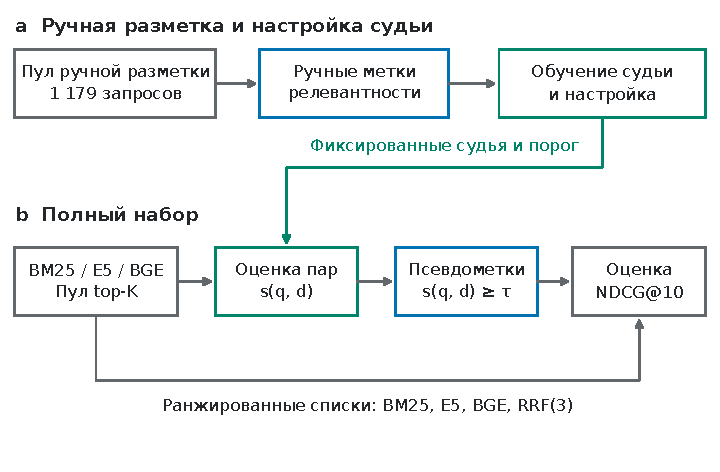
\includegraphics[width=\textwidth]{protocol_ru.pdf}
\caption{Этапы ручной и автоматической разметки. Человеческие оценки служат для обучения судьи; поисковые системы предоставляют фрагменты-кандидаты.}
\label{fig:protocol}
\end{figure}

\subsection{Контролируемые пулы и объединение рангов}
\label{sec:pool-method}

Пусть \(L_m(q)\) обозначает сохранённое ранжирование системы \(m\) для запроса \(q\). Для расширенного набора запросов пул глубины \(K\) определяется как
\begin{equation}
P_q^{(K)}=\bigcup_{m\in\{\mathrm{BM25,E5,BGE}\}}\mathrm{TopK}(L_m(q)),
\quad K\in\{10,30,50,100,200\}.
\label{eq:pool}
\end{equation}
Дубликаты удаляются по идентификатору фрагмента. Сохранённая оценка судьи относится к паре «запрос--фрагмент» и повторно используется на всех глубинах; расширение пула её не меняет. Множество псевдорелевантных фрагментов: \(R_q^{(K)}=\{d\in P_q^{(K)}:\hat y(q,d)=1\}\).

Трёхстороннее объединение RRF(3) использует только BM25, E5 и BGE:
\begin{equation}
\mathrm{RRF}_K(d\mid q)=\sum_{m:d\in\mathrm{TopK}(L_m(q))}\frac{1}{60+\mathrm{rank}_m(d,q)}.
\label{eq:rrf}
\end{equation}
Отсутствующий документ даёт нулевой вклад от данного входного списка. При равенстве оценок документы упорядочиваются по возрастанию числового идентификатора фрагмента. В ручном эксперименте доступны списки глубины десять. В эксперименте на полном наборе меняются и глубина пула, и глубина входных списков \(\mathrm{RRF}_K\). Это два разных изменения: собственные первые десять результатов поисковых систем фиксированы, тогда как первая десятка объединённого списка может измениться при подаче более глубоких списков. В дополнительном анализе глубина входа объединения фиксирована на 200, меняется только пул оценки.

\subsection{Метрики и статистические проверки}
\label{sec:metrics}

NDCG@10 представляет собой нормированную дисконтированную накопленную полезность на первых десяти позициях. При бинарной релевантности числитель придаёт больший вес релевантным фрагментам на более высоких позициях. Для фиксированных пула и набора меток
\begin{align}
\mathrm{DCG}@10(q,m)&=\sum_{i=1}^{10}\frac{y(q,L_m(q)_i)}{\log_2(i+1)},\\
\mathrm{IDCG}@10(q)&=\sum_{i=1}^{\min(10,|R_q|)}\frac{1}{\log_2(i+1)},\\
\mathrm{NDCG}@10(q,m)&=\frac{\mathrm{DCG}@10(q,m)}{\mathrm{IDCG}@10(q)}.
\label{eq:ndcg}
\end{align}
Идеальный знаменатель одинаков для всех систем при данном запросе и наборе меток. Он вычисляется по всем положительным оценкам в пуле, а не только по положительным результатам конкретной системы. Если система не нашла положительных фрагментов, запрос получает нулевую оценку. Если положительных оценок нет во всём пуле, NDCG для всех систем определяется как ноль. Все средние вычислены на одном наборе запросов, без отдельной для каждой системы фильтрации по успешности поиска. Неразмеченные фрагменты сохраняют свои позиции и дают нулевой вклад. Это оценки по пулам, а не показатели общекорпусного рейтинга систем.

Ручное сравнение до и после доразметки использует все 1\,179 запросов. Мы вычисляем парные разности по запросам, 95\% перцентильные бутстреп-интервалы по 5\,000 перевыборок и двусторонние парные тесты со случайной сменой знака по 10\,000 рандомизаций. Оценка Монте-Карло использует поправку \((b+1)/(B+1)\), где \(b\) обозначает число рандомизированных эффектов, не меньших наблюдаемого по абсолютной величине. Для четырёх тестов эффекта ручной доразметки также применяется поправка Бонферрони с семейным уровнем значимости 0.05. Для интервалов на полном наборе настройки перевыборки приведены при таблице~\ref{tab:fullset}; единицей перевыборки остаётся запрос, а не отдельный фрагмент.

\section{Результаты ручной доразметки}
\label{sec:manual-results}

Таблица~\ref{tab:manual-results} сравнивает одинаковые ранжирования по официальной неполной разметке и дополнительным человеческим оценкам. Каждое изменение одновременно является разностью средних и средней парной разностью, поскольку оба столбца охватывают одни и те же 1\,179 запросов. Изменения характеризуют чувствительность оценки к охвату разметки, а не переобучение поисковых моделей.

\begin{table}[t]
\caption{NDCG@10 в пуле до и после ручной доразметки на всех 1\,179 запросах; это не оценки по полному корпусу. $\Delta$: ручная минус исходная разметка; интервалы: парный 95\%-й бутстреп.}
\label{tab:manual-results}
\centering\small
\begin{tabularx}{\textwidth}{@{}Lrrrr@{}}
\toprule
Система & Исходная & Ручная & $\Delta$ & 95\% ДИ \\
\midrule
BM25 & 0.248 & 0.644 & +0.396 & [0.372, 0.419] \\
E5 & 0.488 & 0.879 & +0.391 & [0.365, 0.417] \\
BGE & 0.433 & 0.828 & +0.395 & [0.369, 0.419] \\
RRF(3) & 0.459 & 0.854 & +0.395 & [0.371, 0.419] \\
\bottomrule
\end{tabularx}
\end{table}


Все четыре средних изменения положительны, их доверительные интервалы не включают ноль, а парные тесты дают \(p<0.001\), в том числе с поправкой на множественные проверки. По ручной разметке E5 имеет наибольшую NDCG среди трёх систем поиска только по запросу. RRF(3) находится между E5 и BGE и в этом ручном эксперименте не превосходит E5. Эти сравнения относятся к системам поиска только по запросу и их объединению; вспомогательные каналы разметки в сравнении систем не участвуют.

\begin{figure}[t]
\centering
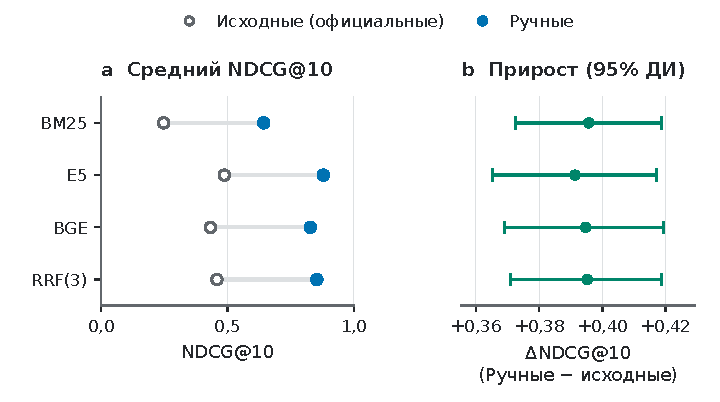
\includegraphics[width=\textwidth]{manual_effect_ru.pdf}
\caption{Оценка ручного пула на одних и тех же 1\,179 запросах с общим идеальным знаменателем. Интервалы парного эффекта отражают неопределённость по запросам, а не вариацию независимо обученных моделей.}
\label{fig:manual-effect}
\end{figure}

После исключения 23 запросов с неинтерпретированными категориями или отсутствующим текстом остаётся 1\,156 запросов. NDCG по ручной разметке составляет 0.644 для BM25, 0.879 для E5, 0.828 для BGE и 0.855 для RRF(3); порядок систем сохраняется. Эта проверка ограничивает влияние указанных проблем качества данных на ручное сравнение, но не заменяет повторной оценки неоднозначных меток или исследования согласия между асессорами.

\subsection{Согласие судьи с разметкой и его интерпретация}
\label{sec:judge-results}

Таблица~\ref{tab:judge-results} разделяет зафиксированный валидационный результат базовой модели и согласие, пересчитанное по сохранённым оценкам дообученной модели. На отложенных тестовых запросах дообученный судья достигает ROC-AUC \JudgeTestAuc{}, F1 \JudgeTestFOne{}, точности (precision) \JudgeTestPrecision{} и полноты (recall) \JudgeTestRecall{}. После валидации порог фиксирован.

\begin{table}[t]
\caption{Качество судьи. AUC базовой модели взят из записи обучения; метрики дообученной модели пересчитаны по сохранённым оценкам. P: точность; R: полнота.}
\label{tab:judge-results}
\centering\small
\begin{tabularx}{\textwidth}{@{}Lrrrrrr@{}}
\toprule
Модель / выборка & Запр. & Пар & AUC & F1 & P & R \\
\midrule
Base / валидация & 177 & 5\,122 & 0.865 & -- & -- & -- \\
Дообуч. / валидация & 177 & 5\,122 & 0.908 & 0.868 & 0.829 & 0.912 \\
Дообуч. / тест & 177 & 5\,002 & 0.907 & 0.875 & 0.851 & 0.902 \\
\bottomrule
\end{tabularx}
\end{table}


Для дополнительной проверки поведения судьи при исходной разметке весь ручной пул кандидатов ранжируется по его оценке на 177 отложенных запросах. NDCG@10 составляет \JudgeHeldoutOriginalNdcg{} по официальным меткам и \JudgeHeldoutHumanNdcg{} по ручным. Это переранжирование при условии уже обогащённого пула, а не качество первичного поиска судьи по всему корпусу; оно не устанавливает превосходство над всеми системами отбора кандидатов.

\begin{figure}[t]
\centering
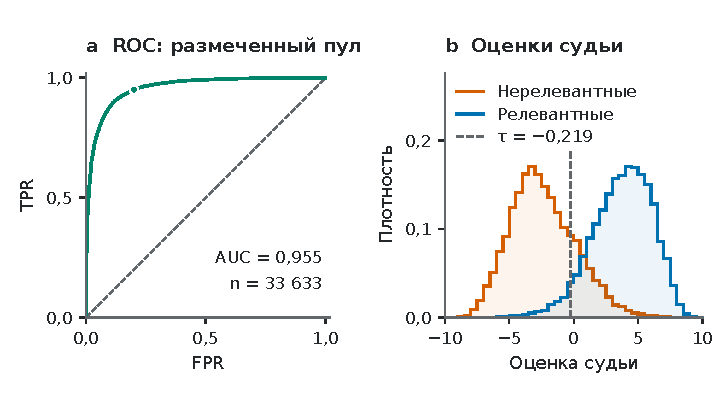
\includegraphics[width=\textwidth]{judge_diagnostics_ru.pdf}
\caption{Диагностика оценок на парах ручного пула со стандартными метками и непустыми текстами. Пул включает обучающие запросы; рисунок не является независимой оценкой на тестовой выборке. Согласие на отложенных данных отдельно приведено в таблице~\ref{tab:judge-results}.}
\label{fig:judge}
\end{figure}

Применение формулы~\ref{eq:judge} ко всем сохранённым оценкам ручного пула даёт \JudgePositiveCount{} псевдоположительных пар, или \JudgeMeanRel{} на запрос, против \HumanPositiveCount{} положительных ручных оценок. Большее число предсказаний не свидетельствует о более точной разметке: необходимо учитывать и ложноположительные, и ложноотрицательные результаты. Основой проверки качества судьи остаются человеческие оценки; псевдометки служат экспериментальным инструментом исследования более крупных пулов.

\section{Псевдоразметка полного набора и глубина пула}
\label{sec:fullset}

Для полного набора метки восстанавливаются по сохранённым оценкам пар «запрос--фрагмент» с одинаковым порогом на всех глубинах. Таблица~\ref{tab:fullset} показывает охват кандидатов, число положительных меток и метрики ранжирования на общем наборе запросов. При глубине десять среднее число кандидатов на запрос равно \FullPoolSmall{}, псевдоположительных фрагментов \FullPositiveSmall{}. При глубине 200 соответствующие значения составляют \FullPoolLarge{} и \FullPositiveLarge{}.

\begin{table}[t]
\caption{Оценка по псевдометкам на всех 101\,093 запросах, включая пулы без положительных меток. Величина пула и число положительных меток усреднены по запросам; для систем приведён NDCG@10. Глубина входа RRF равна $K$. Парные интервалы и тесты используют 2\,000 повторов, seed 20260914.}
\label{tab:fullset}
\centering\small
\begin{tabularx}{\textwidth}{@{}Lrrrrrr@{}}
\toprule
$K$ & Пул & Полож. & BM25 & E5 & BGE & RRF(3) \\
\midrule
10 & 21.88 & 14.19 & 0.649 & 0.871 & 0.851 & 0.852 \\
30 & 65.85 & 33.71 & 0.638 & 0.851 & 0.832 & 0.862 \\
50 & 110.36 & 49.42 & 0.635 & 0.847 & 0.829 & 0.856 \\
100 & 222.91 & 81.02 & 0.633 & 0.844 & 0.825 & 0.851 \\
200 & 451.54 & 128.64 & 0.632 & 0.842 & 0.824 & 0.850 \\
\bottomrule
\end{tabularx}
\end{table}


RRF(3) уступает E5 при $K=10$ (0.852 против 0.871), но превосходит его при всех четырёх больших исследованных глубинах. При $K=200$ парная разность равна $+0.0088$, 95\%-й ДИ $[0.0082, 0.0095]$. Для всех пяти сравнений нескорректированное парное $p<0.001$; они также проходят поправку Бонферрони для пяти проверок при уровне 0.05. Это согласие с фиксированным судьёй, а не независимо подтверждённое превосходство по человеческим оценкам.

DCG первых десяти результатов отдельных поисковых моделей не меняется при росте $K$: изменяется лишь общий идеальный знаменатель. Более глубокие входные списки RRF, напротив, могут менять само итоговое ранжирование. При фиксированной глубине входа RRF, равной 200, NDCG составляет 0.805 при глубине разметки десять и 0.850 при глубине 200. В первом случае 145\,643 возвращённых пар находятся вне размеченного пула и получают нулевой вклад. Эта проверка отделяет неполноту разметки от усечения входов слияния.

Все 1\,179 запросов ручной части входят в большой набор, поэтому он не является полностью независимой тестовой выборкой. Их исключение оставляет 99\,914 запросов. При глубине 200 разность RRF минус E5 сохраняется: $+0.0088$ (95\%-й ДИ $[0.0080, 0.0094]$); направления всех пяти сравнений также не меняются. Проверены оценки для всех 45\,647\,587 пар без пропусков; при глубине 200 у 1\,592 запросов нет положительного предсказания.


\begin{figure}[t]
\centering
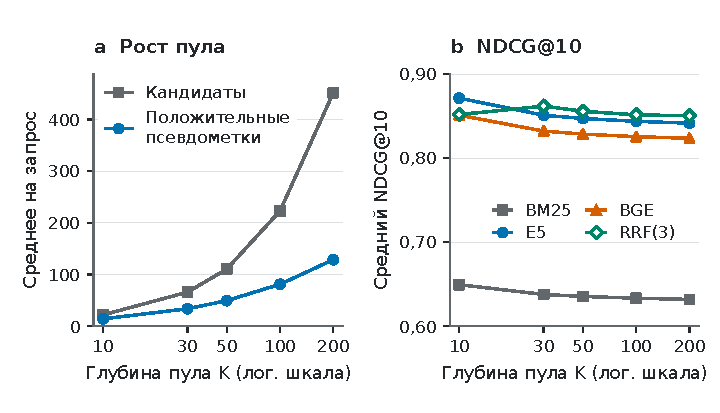
\includegraphics[width=\textwidth]{fullset_pooling_ru.pdf}
\caption{Охват кандидатов, плотность псевдоразметки и поведение ранжирования при изменении глубины пула. На каждой глубине все системы используют одинаковую разметку и набор запросов. Усечение входных списков RRF рассматривается отдельно от размера пула разметки.}
\label{fig:fullset}
\end{figure}

Условное среднее число положительных меток при глубине 200 равно \FullPositiveLargeConditional{}, если исключить запросы без положительных предсказаний. Безусловное среднее равно \FullPositiveLarge{}. В обоих случаях общее число положительных меток одинаково, но знаменатели различаются. Поэтому утверждение «около 130 релевантных документов на запрос» требует указать пул кандидатов, судью, порог и учёт запросов без положительных меток. Это не оценка истинной плотности релевантных документов во всём корпусе.

\section{Ограничения и обсуждение}
\label{sec:discussion}

\paragraph{Разметка и формирование пула.}
Ручная оценка охватывает отобранных кандидатов, а не весь корпус. Использование известного ответа при подготовке кандидатов и ручной оценке обогащает пул и может привязывать интерпретацию релевантности к этому ответу. Это помогает находить альтернативные ответы, но может недостаточно представлять другие допустимые трактовки неоднозначного запроса. Точное установление роли каждого вспомогательного канала и независимая оценка согласия между асессорами выходят за рамки контролируемого сравнения. Нестандартные метки и пустые тексты описаны; проверка чувствительности с исключением запросов не устраняет всех возможных ошибок разметки.

\paragraph{Качество судьи.}
MiniLM является базовой cross-encoder-моделью. Согласие на отложенных данных обосновывает её использование для контролируемого анализа по оценкам, но псевдометки не являются эталонной человеческой разметкой. Диагностику, включающую обучающие запросы, нельзя смешивать с оценками на отложенных данных. Обработка неинтерпретированных категорий при исходном обучении составляет ещё одно ограничение. Более крупные или новые модели переранжирования, включая cross-encoder-варианты BGE, могут давать другие метки и результаты сравнения систем.

В этом эксперименте автоматический судья получает только запрос и кандидата. Это намеренно ограниченная базовая модель, а не требование предоставлять асессору ту же информацию, что и поисковой системе. Известный релевантный ответ допустимо передать судье, не передавая его поисковой модели. Поэтому в дальнейшем судья с опорным ответом должен использовать формат «запрос, известный релевантный ответ, фрагмент-кандидат» и оцениваться по отложенным человеческим суждениям. Сравнение с такой моделью здесь не заявляется.

\paragraph{Оценка и переносимость.}
И определение IDCG, и учёт запросов без положительных меток влияют на средние показатели. Расширение пула может менять доступную разметку, а более глубокие входные списки RRF дополнительно меняют ранжирование. Эти эффекты следует сообщать раздельно. Более близкое согласие с конкретным судьёй также не позволяет по псевдоразметке заключить, что модель универсально лучше.

Наши выводы относятся к английской MS MARCO и исследованным пулам. Различия провайдеров, языков, намерений пользователей и предметных областей документов могут менять результаты. Переносимость между географическими или социальными группами не проверялась, репрезентативность для населения не заявляется. Естественным следующим шагом является оценка на разнородных коллекциях, таких как BEIR \cite{thakur2021beir}; одного многоязычного перевода недостаточно для установления демографического охвата.

\section{Заключение}
\label{sec:conclusion}

Углублённая доразметка в этой работе означает расширение охвата человеческих оценок релевантности внутри заданного пула кандидатов. На 1\,179 запросах дополнительные оценки увеличивают среднее число положительных меток с \OriginalMeanRel{} до \HumanMeanRel{}. Измеренная NDCG@10 растёт для BM25, E5, BGE и RRF(3), когда одинаковые ранжирования и набор запросов оцениваются по более плотной разметке. В ручном эксперименте E5 остаётся лучшей из трёх систем поиска только по запросу.

Судья MiniLM позволяет провести более масштабный контролируемый анализ псевдоразметки и достигает ROC-AUC \JudgeTestAuc{} на отложенных данных. Его вход намеренно ограничен текстами запроса и кандидата. В дальнейшем следует сравнить более сильные cross-encoder-модели и судью с опорным релевантным ответом в формате «запрос, известный релевантный ответ, фрагмент-кандидат». Такое исследование проверит пользу опорной информации для оценки, не предполагая оптимальности нынешней базовой модели.

Глубина пула необходима для интерпретации результатов на полном наборе. По меткам судьи RRF(3) уступает E5 при глубине входа десять, но превосходит его при четырёх больших исследованных глубинах. Число положительных меток зависит от того, какие документы оцениваются; объединение рангов также зависит от глубины входных списков. Ни большое число псевдоположительных меток, ни преимущество объединения нельзя переносить на другие условия оценки без проверки этих условий.

Дополнительная ручная разметка и автоматическая псевдоразметка полезны как исследовательские инструменты при явном описании отбора кандидатов, нормировки, порога и оцениваемой совокупности запросов. Поэтому переоценка MS MARCO включает и расширение охвата разметки, и определение согласованной процедуры измерения; переносимость за пределы этой коллекции требует дальнейшей эмпирической проверки.

\begin{thebibliography}{99}
\bibitem{bajaj2016msmarco}
Bajaj, P., Campos, D., Craswell, N., et al.: MS MARCO: A Human Generated MAchine Reading COmprehension Dataset. arXiv:1611.09268 (2016).
\url{https://arxiv.org/abs/1611.09268}

\bibitem{msmarco_datasets}
Microsoft: MS MARCO datasets and passage-ranking resources.
\url{https://microsoft.github.io/msmarco/Datasets}. Accessed 14 September 2026.

\bibitem{kwiatkowski2019naturalquestions}
Kwiatkowski, T., Palomaki, J., Redfield, O., et al.: Natural Questions: A Benchmark for Question Answering Research. Transactions of the Association for Computational Linguistics 7 (2019).
\url{https://doi.org/10.1162/tacl_a_00276}

\bibitem{chapelle2011yahoo}
Chapelle, O., Chang, Y.: Yahoo! Learning to Rank Challenge Overview. In: Proceedings of the Learning to Rank Challenge. PMLR 14, pp. 1--24 (2011).
\url{https://proceedings.mlr.press/v14/chapelle11a.html}

\bibitem{yandex2013personalized}
Yandex: Personalized Web Search Challenge. Kaggle competition (2013--2014).
\url{https://www.kaggle.com/c/yandex-personalized-web-search-challenge}.
Accessed 14 September 2026.

\bibitem{bonifacio2022mmarco}
Bonifacio, L., Jeronymo, V., Abonizio, H.Q., Campiotti, I., Fadaee, M., Lotufo, R., Nogueira, R.: mMARCO: A Multilingual Version of MS MARCO Passage Ranking Dataset. arXiv:2108.13897 (2021).
\url{https://arxiv.org/abs/2108.13897}

\bibitem{2025rusbeir}
Building Russian Benchmark for Evaluation of Information Retrieval Models. Computational Linguistics and Intellectual Technologies (2025).
\url{https://arxiv.org/abs/2504.12879}

\bibitem{thakur2021beir}
Thakur, N., Reimers, N., R\"uckl\'e, A., Srivastava, A., Gurevych, I.: BEIR: A Heterogeneous Benchmark for Zero-shot Evaluation of Information Retrieval Models. Proceedings of the Neural Information Processing Systems Track on Datasets and Benchmarks 1 (2021).
\url{https://arxiv.org/abs/2104.08663}

\bibitem{robertson2009bm25}
Robertson, S.E., Zaragoza, H.: The Probabilistic Relevance Framework: BM25 and Beyond. Foundations and Trends in Information Retrieval 3(4), 333--389 (2009).

\bibitem{wang2022e5}
Wang, L., Yang, N., Huang, X., Jiao, B., Yang, L., Jiang, D., Majumder, R., Wei, F.: Text Embeddings by Weakly-Supervised Contrastive Pre-training. arXiv:2212.03533 (2022).
\url{https://arxiv.org/abs/2212.03533}

\bibitem{xiao2023cpack}
Xiao, S., Liu, Z., Zhang, P., Muennighoff, N., Lian, D., Nie, J.-Y.: C-Pack: Packed Resources for General Chinese Embeddings. arXiv:2309.07597 (2023).
\url{https://arxiv.org/abs/2309.07597}

\bibitem{nogueira2019bert}
Nogueira, R., Cho, K.: Passage Re-ranking with BERT. arXiv:1901.04085 (2019).
\url{https://arxiv.org/abs/1901.04085}

\bibitem{cormack2009rrf}
Cormack, G.V., Clarke, C.L.A., B\"uttcher, S.: Reciprocal Rank Fusion outperforms Condorcet and Individual Rank Learning Methods. In: Proceedings of SIGIR, pp. 758--759 (2009).

\bibitem{bruch2023fusion}
Bruch, S., Gai, S., Ingber, A.: An Analysis of Fusion Functions for Hybrid Retrieval. arXiv:2210.11934 (2022; revised 2023).
\url{https://arxiv.org/abs/2210.11934}

\bibitem{voorhees2005trec}
Voorhees, E.M., Harman, D.K. (eds.): TREC: Experiment and Evaluation in Information Retrieval. MIT Press (2005).

\bibitem{wang2020minilm}
Wang, W., Wei, F., Dong, L., Bao, H., Yang, N., Zhou, M.: MiniLM: Deep Self-Attention Distillation for Task-Agnostic Compression of Pre-Trained Transformers. Advances in Neural Information Processing Systems 33, 5776--5788 (2020).

\bibitem{reimers2019sentencebert}
Reimers, N., Gurevych, I.: Sentence-BERT: Sentence Embeddings using Siamese BERT-Networks. In: Proceedings of EMNLP-IJCNLP, pp. 3982--3992 (2019).
\url{https://doi.org/10.18653/v1/D19-1410}
\end{thebibliography}

\clearpage
\section*{Замечания рецензентов и ответы авторов}
\label{sec:responses}
\noindent Заявка 90. Редакция для DAMDID 2026 от 14 сентября 2026 года.

\paragraph{Рецензент 1: терминология и примеры (скорее принять).}
\emph{Замечание, краткий пересказ русского оригинала.} Статья содержит необходимые разделы исследования, но смысл углублённой доразметки недостаточно ясен. Рецензент просит привести конкретные примеры и пояснения, делающие основные понятия доступными читателям, менее знакомым с темой.

\emph{Ответ.} Во введении и разделе~\ref{sec:annotation} дано операциональное определение: углублённая доразметка расширяет человеческие оценки в отобранном пуле, а не увеличивает глубину нейронной сети и не охватывает весь корпус. Раздел~\ref{sec:example} и таблица~\ref{tab:example} содержат реальный запрос MS MARCO, идентификаторы фрагментов, сокращённые описания их содержания и статус релевантности до и после разметки. Пояснение показывает, почему верный, но неразмеченный ответ не даёт вклада в метрику при неполных qrels. Изменение измеренного качества явно отделено от улучшения неизменных поисковых моделей; объяснены qrels, формирование пула, псевдометки и вход судьи. Эти пояснения включены и в русскую версию.

\paragraph{Рецензент 2: общая оценка (принять).}
\emph{Замечание, краткий пересказ.} Рецензент считает задачу улучшения набора данных важной, результаты ценными, стратегию обоснованной и поддерживает публикацию полноформатной статьи.

\emph{Ответ.} Благодарим рецензента за положительную оценку. Конкретных дополнительных изменений не запрошено. В новой редакции сохранён фокус на охвате разметки релевантности и добавлены изложенные здесь пояснения и методологические уточнения.

\paragraph{Рецензент 3: другие провайдеры и универсальность (уверенно принять).}
\emph{Замечание, краткий пересказ.} Есть ли аналоги MS MARCO у Google, Yandex или Yahoo? Насколько универсальна MS MARCO с учётом возможных различий в использовании поисковых систем между странами и социальными группами? Рецензент предлагает обосновать выбор MS MARCO во введении.

\emph{Ответ.} В разделе~\ref{sec:intro} рассмотрены Natural Questions от Google, Learning to Rank Challenge от Yahoo! и Personalized Web Search Challenge от Yandex со ссылками на первоисточники. Разграничены ответы на вопросы по текстам, ранжирование по векторам признаков и анонимизированные журналы взаимодействий; эти наборы не рассматриваются как взаимозаменяемые. Выбор MS MARCO объяснён доступностью текстов, неполной разметкой, устоявшимися средствами оценки и предобученными моделями. Разделы~\ref{sec:related} и \ref{sec:discussion} обсуждают межколлекционную оценку и прямо указывают, что переносимость между странами и социальными группами не проверялась. Демографическая репрезентативность или универсальная применимость результатов не заявляются.

\paragraph{Дополнительные методологические исправления.}
При проверке установлено, что прежний расчёт использовал отдельный идеальный знаменатель для каждой системы и исключал запросы без найденного положительного фрагмента. Мы перешли к общему IDCG по пулу и единой совокупности запросов, пересчитали таблицы ранжирования, парные эффекты, доверительные интервалы и рисунки. Базовая разметка теперь непосредственно использует официальные qrels подвыборки разработки: в ручном пуле 1\,243 положительные пары; медиана числа ручных положительных оценок исправлена на 17. Псевдометки единообразно восстановлены по исходным оценкам и сохранённому порогу: в ручном пуле 22\,206 положительных пар. Явно указаны вспомогательные источники пула, RRF ограничен тремя названными системами поиска только по запросу, а глубина его входных списков отделена от глубины пула оценки. Эти изменения затрагивают численные результаты и границы выводов, поэтому представлены явно, а не как чисто редакционные правки. Качественный вывод о росте измеренной NDCG после ручной доразметки сохраняет подтверждение при исправленном протоколе.

Направление сравнения объединённой выдачи на полном наборе изменилось относительно прежней версии: восстановленный RRF(3) уступает E5 при глубине десять и превосходит его при четырёх больших исследованных глубинах. Результат сохраняется после исключения всех запросов ручной подвыборки. Раздел~\ref{sec:fullset} и заключение исправлены соответственно; прежнее утверждение о поведении объединения не сохраняется.

\end{document}
